%----------------------------------------------------------------------------
\chapter{Megjelenítési réteg}

\section{Alacsony szintű grafikai kihívások}

A gépközeli grafikai interfészek használatával elveszítünk bizonyos egyszerűsített műveleteket, például a komplex alakzatok kódból történő közvetlen felrajzolását. A legtöbb grafikus kártya bizonyos feltételezésekkel él a rajta átfutó adatok feldolgozásakor, és így ezek teljesülésére sem képes garanciát vállalni a programunk. A libGDX kész megoldások helyett erős alapokat biztosít, amivel a fejlesztő saját döntése szerint implementálhatja vagy eseti alapon figyelmen kívül hagyhatja a GPU\footnote{Graphics Processing Unit} írott-íratlan igényeit; pár példát bemutatok ezekből.

\subsection{Háromszögelés, fülvágó algoritmus}

A két dimenziós háromszög a leggyakoribb elemi alakzat, amit minden platform grafikus interfésze feltétel nélkül támogat; célszerű lenne tehát a modelleket ezek összességére redukálni.

Geometriailag intuitív felosztó eljárás a fülvágó algoritmus (ear-clipping algorithm). Fül alatt olyan háromszöget értünk, amit egy poligon egymást követő három csúcspontja alkot, melyek közül a középső konvex -- tehát az adott pontban a sokszög belső szöge legfeljebb 180 fok ($\pi$ radián).\cite{TriangulationByEarClipping} Az ilyen hármasok által határolt terület garantáltan kivonható a poligonéból, mivel definíció szerint nem lehet lyuk vagy kihagyás benne, így nem kell kompenzálni az üres térért. Az eljárás a megmaradt területre megismételhető, és minden lépés egy újabb háromszög alakú részletet fog eredményezni; így a célunkat el is érjük, amikor már mindössze három csúcspont marad.

Az algoritmus célja tehát a fent leírt módszerrel kiszámítani, hogy egy tetszőleges sokszög lefedéséhez milyen módon kell háromszögekké összekötni a kapott vertexeket. Hasznos mellékhatás, hogy ezzel a sokszög területének összegzése is triviálissá válik.

A libGDX esetében a gyakran visszatérő felhasználásnak köszönhetően külön osztály gondoskodik erről (EarClippingTriangulator). Az OpenGL idiómáinak megfelelően lebegőpontos értékekre bontott vektorokat kér bemenetként, eredménye pedig egy egyszerű, indexekből álló lista -- ennek elemei hármasával határoznak meg egy háromszöget.

\begin{lstlisting}[caption=Példa az EarClippingTriangulator felhasználására]
    val floats = baseNodes.flatMap { listOf(it.x, it.z) }.toFloatArray()
    val triangles: ShortArray
    val triangulator = EarClippingTriangulator()
    triangles = triangulator.computeTriangles(floats)
\end{lstlisting}

\subsection{Körbejárási sorrend}

Számos effektus, például megvilágítás alkalmazásához szükséges ismerni az érintett lapok normálvektorát. Matematikai értelemben ez olyan irányt jelent, ami egy felület tetszőleges pontjában merőleges a teljes felületre. Ebből az irányból nézve a felület látszólagos mérete a lehető legnagyobb, mivel köznyelvileg "szemből" látjuk a sokszöget, egyik irányba sincs elforgatva.

Grafikai hatásnak tekinthető az is, hogy egyáltalán látható-e egy poligon. A kirajzolási műveletek számának csökkentése miatt célszerű csak azokat a lapokat számba venni, amiknek a kívánt oldala mutat a kamera felé. Az OpenGL alapértelmezetten "back-face culling" elven működik: a néző csak azokat az alakzatokat látja, amiknek a nézőpontot és az alakzat középpontját összekötő vektor körüli vertex-sorrendje az óramutató járásával ellentétes. Ez a viselkedés az alábbiak szerint módosítható.

\begin{lstlisting}[caption=Példa az OpenGL culling műveleteinek beállításaira libGDX-en keresztül]
    Gdx.gl.glEnable(GL40.GL_CULL_FACE) //bekapcsolás
    Gdx.gl.glCullFace(GL40.GL_BACK) //szűrendő oldal beállítása (hátsó)
    Gdx.gl.glFront(GL40.CW) //körbejárási sorrend megváltoztatása óramutató járása szerintire
\end{lstlisting}

\subsection{A fő szál használata}

A projekt szimulációs részével szemben a megjelenítés nehezen párhuzamosítható. Az OpenGL műveletek általában nem szálbiztosak, egy grafikai kontextust egy időben több helyről használni és módosítani nem érdemes; programunk futása hamar hibára fut.

A grafikus könyvtár a lehető legjobban elrejti az operációs rendszerrel és GPU-val történő kommunikációt, cserébe viszont a fejlesztőnek ügyelnie kell arra, hogy az abszolút szükséges mennyiségre csökkentse a GPU hívásokat. Amíg egyedi kérések feldolgozása történik, a kártya nem tud újabb képkockákat átadni a processzornak, a monitoron tehát "megfagy" az animáció -- ez a későbbi, teljesítményt taglaló fejezetben jól látható.

A programban a fő szálat egyetlen helyen használom jelentősen a képalkotást leszámítva. A vonalakkal meghatározott épületek egyedi modelljét csak a GPU képes legyártani. A végső szoftverben a szálhasználat ütemezése helyett szokásosnak mondható módon betöltő-képernyő jelenik meg új mentés vagy adatcsomag előkészítése közben. Programozási szempontból csupán a meglévő eszköztárra kellett építenem, lambda függvényt készítettem a fő szál kontextusának tetszőleges szálon történő megszerzéséhez.

\begin{lstlisting}[caption=A kirajzoló szál használatát segítő generikus függvény]
private suspend fun <T> runOnRenderThread(block: () -> T): T {
        return suspendCoroutine { continuation ->
            Gdx.app.postRunnable {
                continuation.resume(block())
            }
        }
    }
\end{lstlisting}

\section{Implementáció}
A program grafikus része modulokra bontható. Az épületek bemutatására hivatott interaktív, három dimenziós OpenGL teret csomagoló, főszerepű jeleneten kívül több független, felhasználói kommunikációt megvalósító komponens is létezik.

\section{A fő jelenet}
A grafikus felület egyszerűsített, domborzatot figyelmen kívül hagyó módon ábrázolja az egyes épületeket. Stílusa inspirációt merít a kortárs városépítő videojátékok (SimCity, Cities: Skylines) és a Google Earth kinézetéből. %TODO: felülnézet?
\begin{figure}[!ht]
    \centering
    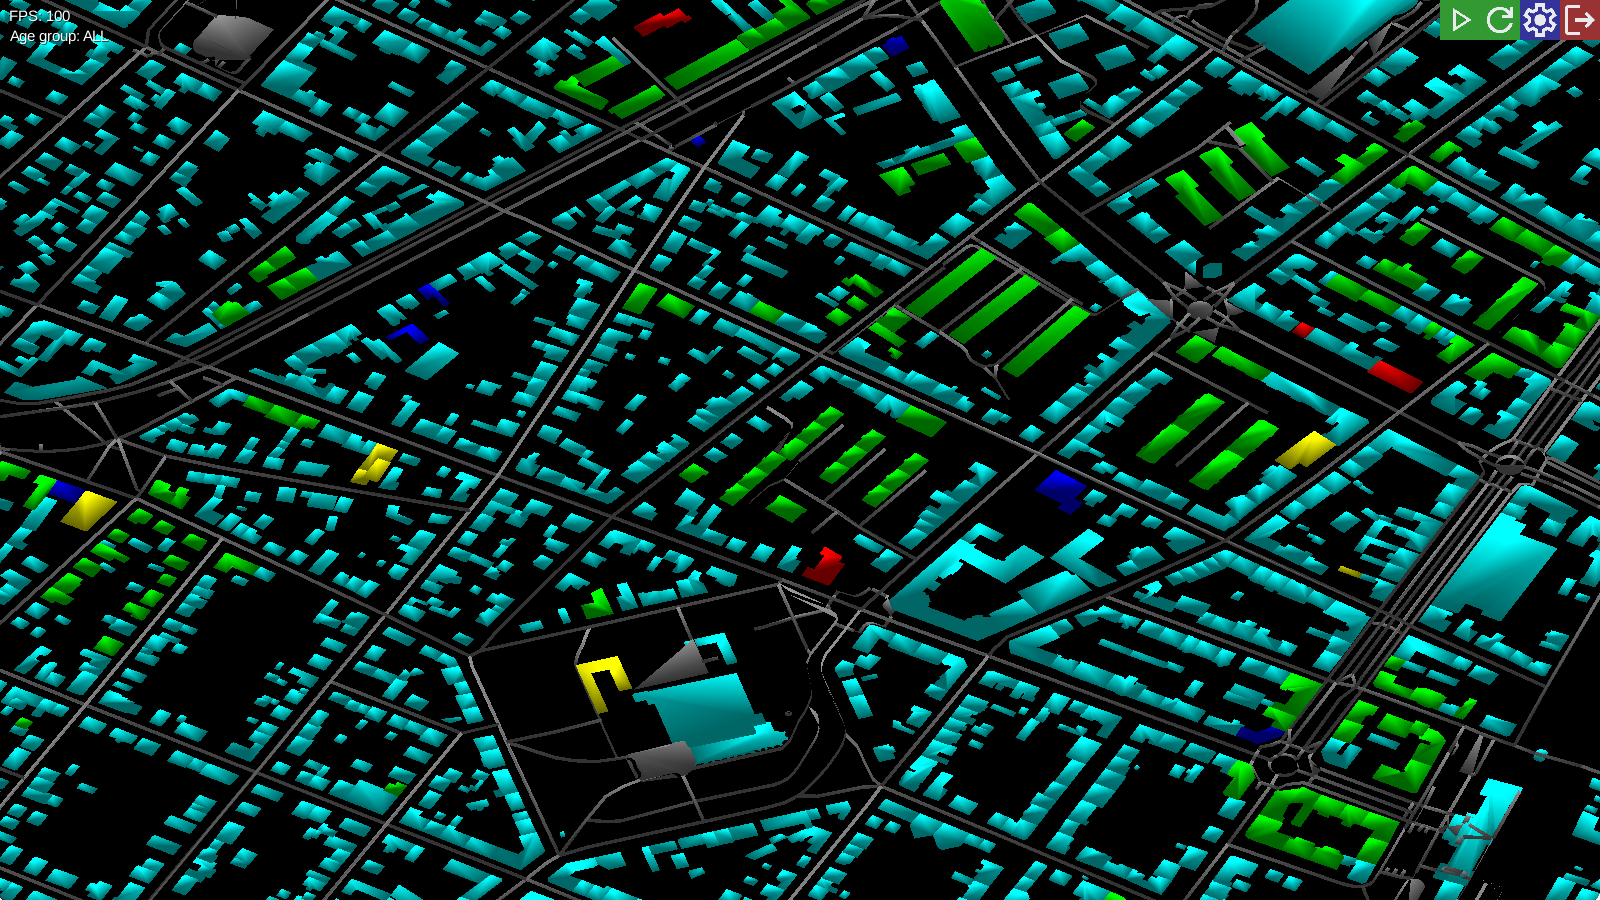
\includegraphics[width=150mm, keepaspectratio]{images/main_graphics_view.png}
    \caption{A játék fő képernyője, "fals 3D" nézettel.}
\end{figure}

\subsection{Egyedi kamera irányítás}

A libGDX jelenetei egyetlen bemenetet kezelő objektumot, vagy azok összességéből készült multiplexert képesek tárolni. Bár egy nagy osztály is kezelhetné a kamera irányítását, valamint az egyéb menüfunkciókat, ezt a két kategóriát külön építettem fel. A grafikus könyvtárban elérhető CameraInputController csak az egérrel végzett forgatást és nagyítást adja hozzá az azt meghívó jelenetnek. Ehelyett saját kamerakezelőt írtam, ami a felülnézet zárolásán kívül négy tengelyes, finomított, lendülettel bíró mozgást ad a játékos kezébe.

\
 Egy komplexum, de akár az azt határoló vonalak által leírt poligon is lehet konkáv, így a teljes modellek felépítéséhez a fülvágó algoritmust használtam.

A backend-ről származó adatokból természetesen nem csak az entitások pozíciója, formája lényeges, az OpenStreetMap adathalmaz alapján csoportosíthatók és színezhetők  
